% Copyright (C) 2017 - Michael Baudin

  \documentclass{beamer}

%\setbeameroption{hide notes}
%\setbeameroption{show notes}
%\setbeameroption{show only notes}

  % Copyright (C) 2012 - EDF R&D - Michael Baudin

% To highlight source code
\usepackage{listings}
\definecolor{darkgreen}{rgb}{0,0.5,0}
\definecolor{violet}{rgb}{0.5,0,1}

\usepackage{lmodern}% http://ctan.org/pkg/lm

\usetheme{Montpellier}
\setbeamertemplate{navigation symbols}{} % Remove navigation
\useoutertheme{infolines}

\usepackage[utf8]{inputenc}
\usepackage[T1]{fontenc}

%\usepackage[french]{babel}
%\uselanguage{French}
%\languagepath{French}

\def\bx{{\bf x}}
\def\RR{\mathbb{R}}

\newcommand{\pyvar}[1]{\texttt{#1}}

\def \ot {OpenTURNS}

\hypersetup{colorlinks=true}

\usepackage{adjustbox}

\title[OpenTURNS]{OpenTURNS release highlights}

\author[OpenTURNS et al.]{
Régis Lebrun, Julien Schueller
}

% \institute[Airbus-EDF-IMACS-ONERA-Phimeca]{
% \inst{1} Airbus
% \inst{2} EDF R\&D. 6, quai Watier, 78401, Chatou Cedex - France, michael.baudin@edf.fr \and %
% \inst{3} IMACS
% \inst{4} ONERA
% \inst{5} Phimeca Engineering. 18/20 boulevard de Reuilly, 75012 Paris - France, schueller@phimeca.com
% }

\date[]{UserDay \#13, 5 June 2020, online event}
%%%%%%%%%%%%%%%%%%%%%%%%%%%%%%%%%%%%%%%%%%%%%%%%%%%%%%%%%%%%%%%%%%%%%%%%%%%%%

  \begin{document}

%%%%%%%%%%%%%%%%%%%%%%%%%%%%%%%%%%%%%%%%%%%%%%%%%%%%%%%%%%%%%%%%%%%%%%%%%%%%%

  \begin{frame}
  \titlepage

  \begin{columns}
  \begin{column}[t]{0.05\textwidth}
        \end{column}
  
    \column{0.10\textwidth}
  \begin{center}

\includegraphics[height=0.04\textheight]{figures/airbus-logo-3d-blue.png}
\end{center}

    \column{0.05\textwidth}
  \begin{center}

\includegraphics[height=0.09\textheight]{figures/logo-edf.jpg}
\end{center}

     \column{0.05\textwidth}
  \begin{center}

\includegraphics[height=0.09\textheight]{figures/imacs-logo.jpg}
\end{center}

    \column{0.10\textwidth}
  \begin{center}

\includegraphics[height=0.05\textheight]{figures/onera-logo.png}
\end{center}

    \column{0.15\textwidth}
  \begin{center}

\includegraphics[height=0.08\textheight]{figures/logo-phimeca.png}
\end{center}

\column{0.01\textwidth}

  \end{columns}

  \end{frame}

\begin{frame}
\frametitle{Overview}

%   \begin{columns}
%     \column{0.6\textwidth}
New features since last year in releases:

\begin{itemize}
\item v1.14: 2019-11-13
\item v1.15: 2020-05-25
\end{itemize}

% \begin{center}
% 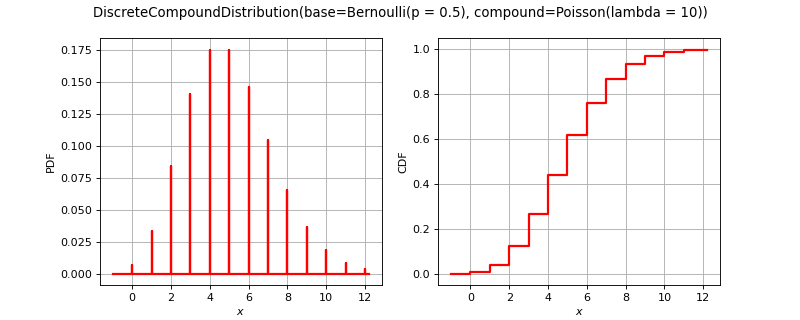
\includegraphics[width=0.8\textwidth]{figures/openturns-DiscreteCompoundDistribution-1.png}
% \end{center}
%     \column{0.4\textwidth}

% 	\begin{center}
% 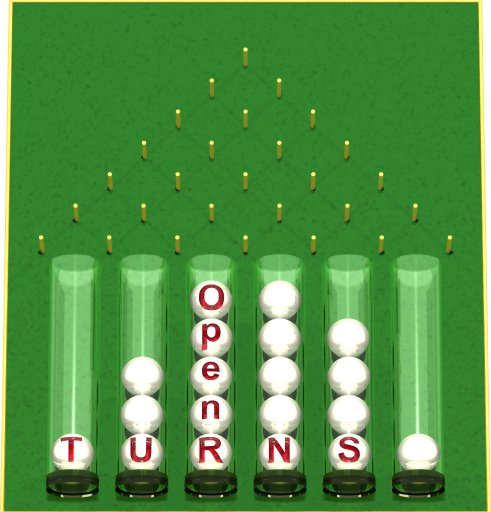
\includegraphics[width=0.9\textwidth]{figures/logo-ot}
% \end{center}

% 	\end{columns}
\end{frame}
  
%%%%%%%%%%%%%%%%%%%%%%%%%%%%%%%%%%%%%%%%%%%%%%%%%%%%%%%%%%%%%%%%%%%%%%%%%%%%%



\begin{frame}
\frametitle{Contents}
\tableofcontents
\end{frame}

%%%%%%%%%%%%%%%%%%%%%%%%%%%%%%%%%%%%%%%%%%%%%%%%%%%%%%%%%%%%%%%%%%%%%%%%%%%%%
\section{Probabilistic modelling capabilities}

%%%%%%%%%%%%%%%%%%%%%%%%%%%%%%%%%%%%%%%%%%%%%%%%%%%%%%%%%%%%%%%%%%%%%%%%%%%%%

\begin{frame}
\frametitle{New distributions}

%   \begin{columns}
%     \column{0.6\textwidth}

\begin{itemize}
\item SquaredNormal
\item DiscreteCompoundDistribution
\item WeibullMax
\item Pareto
\item MixedHistogramUserDefined
\end{itemize}

\begin{center}
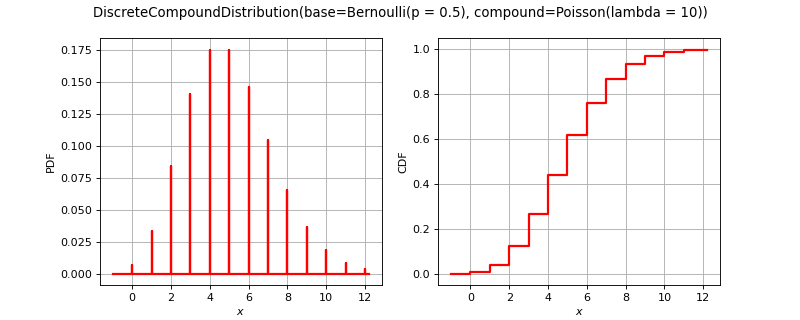
\includegraphics[width=0.8\textwidth]{figures/openturns-DiscreteCompoundDistribution-1.png}
\end{center}
%     \column{0.4\textwidth}

% 	\begin{center}
% 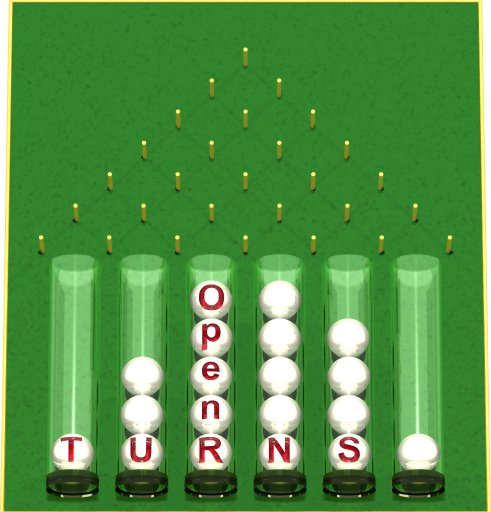
\includegraphics[width=0.9\textwidth]{figures/logo-ot}
% \end{center}

% 	\end{columns}
\end{frame}


\begin{frame}
\frametitle{New estimators}

\begin{itemize}
\item ParetoFactory
\item GeneralizedExtremeValueFactory
\item PlackettCopulaFactory
\item LeastSquaresDistributionFactory (generic service)
\end{itemize}

%     \column{0.4\textwidth}

\begin{center}
  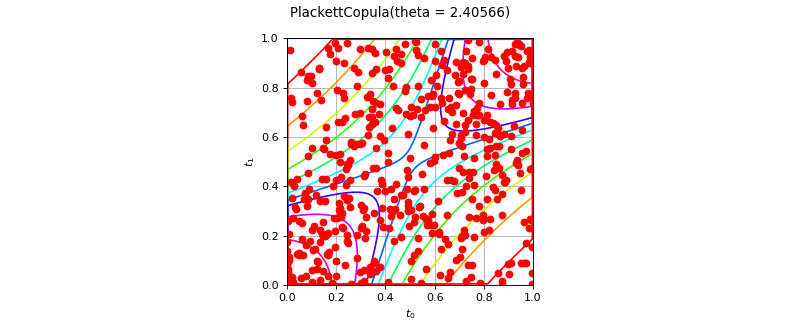
\includegraphics[width=0.9\textwidth]{figures/openturns-PlackettCopulaFactory-1.png}
\end{center}

% 	\end{columns}
\end{frame}

\begin{frame}
\frametitle{New copulas}

  \begin{columns}
      \column{0.4\textwidth}
\begin{itemize}
\item JoeCopula (EV)
\item MarshallOlkinCopula
\item PlackettCopula
\end{itemize}
%     \column{0.4\textwidth}
    \column{0.9\textwidth}
	\begin{center}
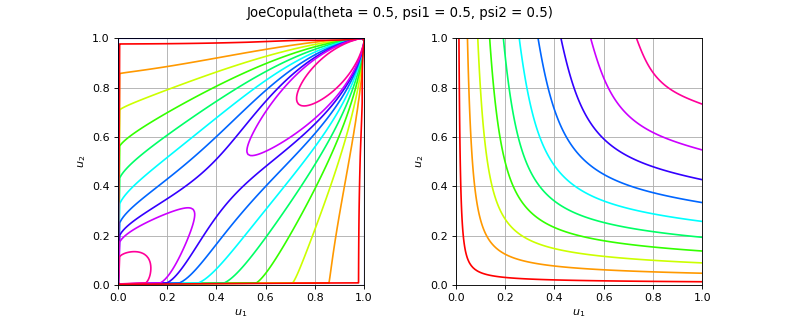
\includegraphics[width=0.5\textwidth]{figures/openturns-JoeCopula-1.png}
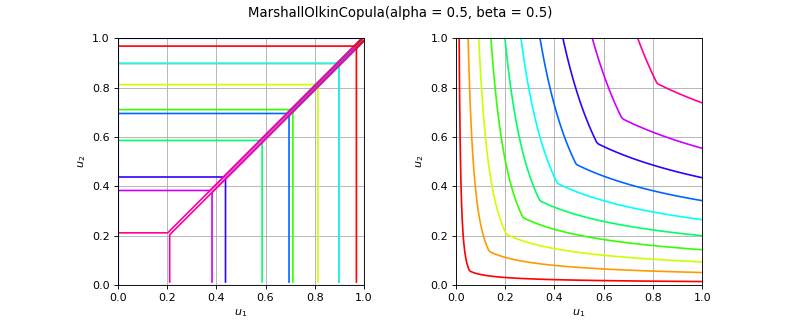
\includegraphics[width=0.5\textwidth]{figures/openturns-MarshallOlkinCopula-1.png}
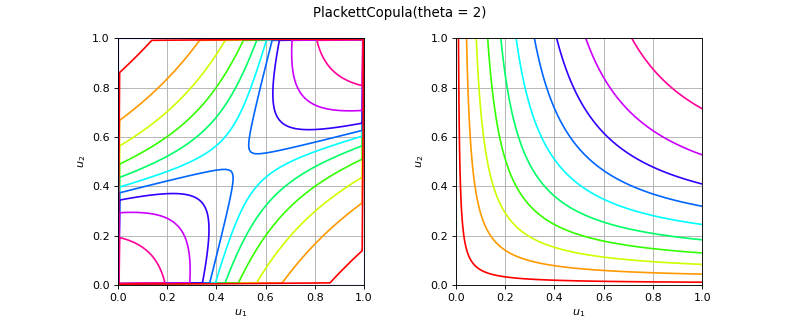
\includegraphics[width=0.5\textwidth]{figures/openturns-PlackettCopula-1.png}
\end{center}

	\end{columns}
\end{frame}

\section{System events}

%%%%%%%%%%%%%%%%%%%%%%%%%%%%%%%%%%%%%%%%%%%%%%%%%%%%%%%%%%%%%%%%%%%%%%%%%%%%%

\begin{frame}
\frametitle{System events}

%   \begin{columns}
%     \column{0.6\textwidth}

\begin{itemize}
\item IntersectionEvent: $E_{sys} = \bigcap_{i=1}^N E_i$
\item UnionEvent: $E_{sys} = \bigcup_{i=1}^N E_i$
\item MultiFORM:\\
  $P(\bigcup_{i=1}^N E_i) = 1 - \Phi_k (\underline{\beta}; \underline{\underline{\rho}})$
\item SystemFORM:\\
  $P(\bigcup_{i=1}^N E_i) = 1 - \Phi_k (\underline{\beta}; \underline{\underline{\rho}})$\\
  $P(\bigcap_{i=1}^N E_i) = \Phi_k (-\underline{\beta}; \underline{\underline{\rho}})$\\
  $P(E_{sys}) = P(\bigcup_{i=1}^N E_i) = \sum_{i=1}^N P(E_i) - \sum_{i < j} P(E_i \cap E_j) + \dots + (-1)^N P(E_1 \cap E_2 \cap \dots \cap E_N)$
\end{itemize}

%     \column{0.4\textwidth}
% 
	\begin{center}
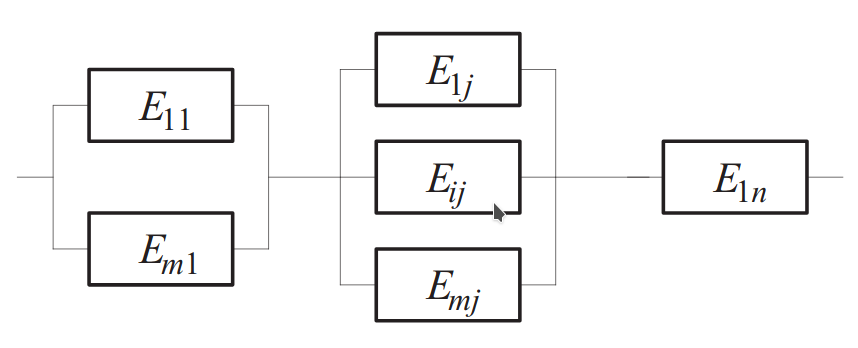
\includegraphics[width=0.7\textwidth]{figures/system.png}
\end{center}
% \end{columns}
\end{frame}


\begin{frame}[containsverbatim]
\frametitle{System events}

\lstset{language=python}

\begin{itemize}
\item Modelisation
\end{itemize}
\begin{lstlisting}
X = ot.RandomVector(ot.Normal(dim))
f1 = ot.SymbolicFunction(['x1', 'x2'], ['(x1+2*x2)^2'])
f2 = ot.SymbolicFunction(['x1', 'x2'], ['(x2+3*x1)^2'])
v1 = ot.CompositeRandomVector(f1, X)
v2 = ot.CompositeRandomVector(f2, X)
e1 = ot.ThresholdEvent(v1, ot.Greater(), 5.0)
e2 = ot.ThresholdEvent(v2, ot.Greater(), 5.0)

# define union/intersection
e3 = ot.IntersectionEvent([e1, e2])
e4 = ot.UnionEvent([e1, e2])
e5 = ot.UnionEvent([e3, e4])

# sample system events
e3.getSample(10)
algo = ot.SubsetSampling(e4)
\end{lstlisting}

\end{frame}



\begin{frame}[containsverbatim]
\frametitle{System events}

\lstset{language=python}

\begin{itemize}
\item Algorithms
\end{itemize}
\begin{lstlisting}
# System-FORM
e5 = ot.IntersectionEvent([e1, e2])
e6 = ot.IntersectionEvent([e3, e4])
e7 = ot.UnionEvent([e5, e6])
solver = ot.AbdoRackwitz()
starting_pt = [0.1] * dim
algo = ot.SystemFORM(e7, event, starting_pt)
algo.run()
result = algo.getResult()
pf = result.getEventProbability()
\end{lstlisting}

\end{frame}




\section{HMAT and OpenTURNS: it works (at last!)}

\begin{frame}[allowframebreaks, containsverbatim]
\frametitle{Discretization of covariance models on large meshes}
There are many contexts in which the discretization of a covariance model over a large mesh is mandatory:
\begin{itemize}
\item to sample a Gaussian process on a large mesh
\item to build a Kriging meta-model from a large dataset
\item to build the Karhunen-Loeve decomposition of a known covariance model on a large mesh
\item ...
\end{itemize}
The resulting matrices are \alert{dense} and \alert{large}, so the first limit is the $\mathcal{O}(N^2)$ memory need ($\sim 30000$ nodes for covariance model of dimension 3 with 64GB of memory).

Using HMAT, the memory footprint is reduced to $\mathcal{O}(N\log N)$, allowing for much larger meshes (tested on a $900720$ nodes mesh with for a covariance model of dimension 3 with 64GB of memory).

Then, the factorization times, which is $\mathcal{O}(N^3)$ with a dense solver (LAPACK) becomes the limiting factor. With HMAT, it drops to $\mathcal{O}(N\log^2 N)$.\\[1em]

\alert{These were the motivation for the introduction of HMAT within OpenTURNS 1.4, nearly 6 years ago... and it didn't worked as expected!}\\[1em]

\begin{itemize}
\item The regularization procedure developed for LAPACK was not adapted to HMAT, resulting into many (many many) factorizations;
\item No compression procedure proposed by the hmat-oss library was adapted to covariance operators.
\end{itemize}

\newpage
These points have been solved in two steps, thanks to Romain Poncet's contributions:
\begin{enumerate}
\item OpenTURNS 1.14: the ability to change the regularization factor without recompressing the matrix, and the automatic computation of a reasonable regularization factor (in OpenTURNS 1.14);
\item OpenTURNS 1.15: The development of the \alert{ACA-random} compression procedure in hmat-oss and its interface in OpenTURNS.
\end{enumerate}

\alert{AND IT WORKS!} Here we compare LAPACK (with OpenBLAS, 4 cores) and hmat-oss (1 core).
\end{frame}

\begin{frame}[allowframebreaks, containsverbatim]
\frametitle{Sampling of a Gaussian process}

\begin{figure}
\begin{center}
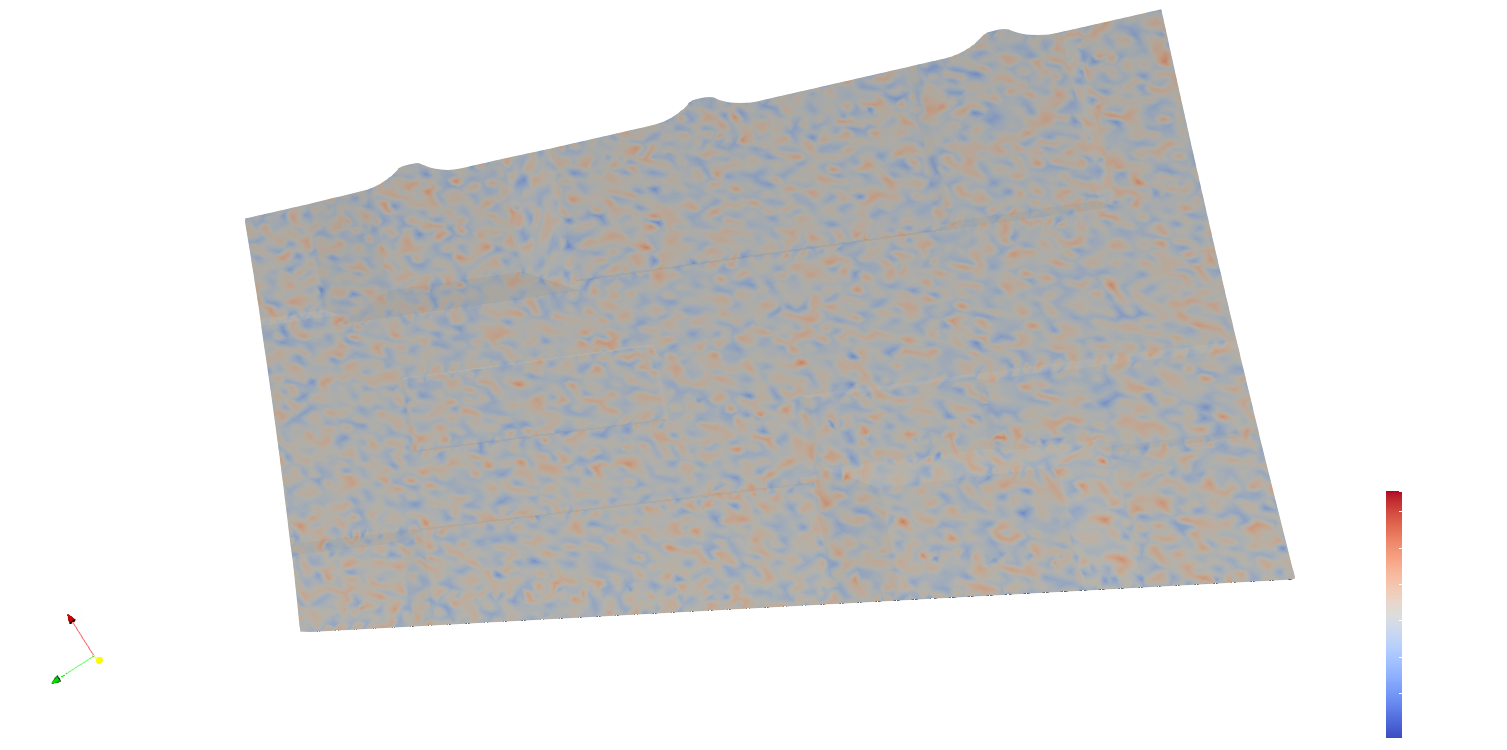
\includegraphics[width=0.5\textwidth]{figures/medium_lapack.png}%
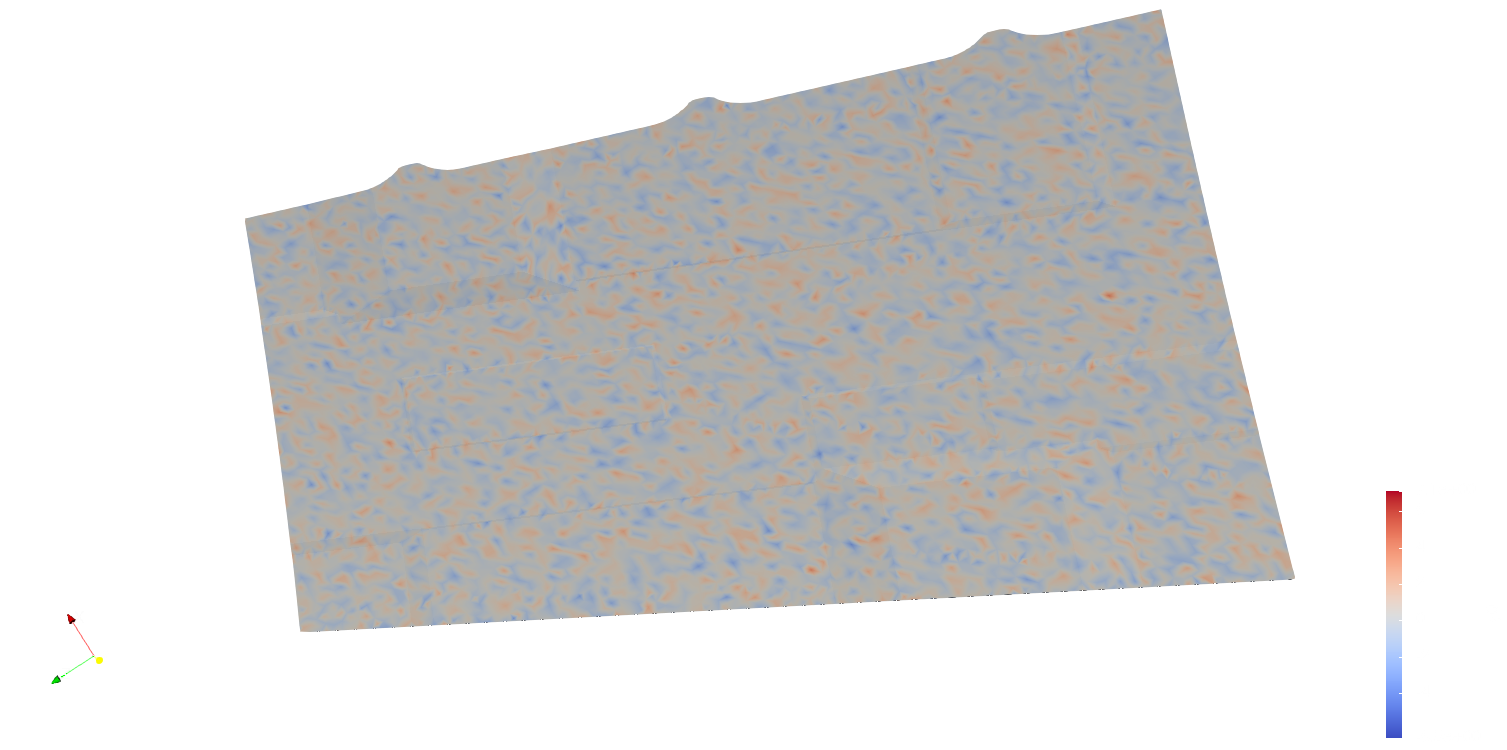
\includegraphics[width=0.5\textwidth]{figures/medium_hmat.png}
\end{center}
\caption{Mat\`ern model, 18292 nodes, LAPACK (left, 188 s), HMAT (right, 90 s)}
\end{figure}

\begin{figure}
\begin{center}
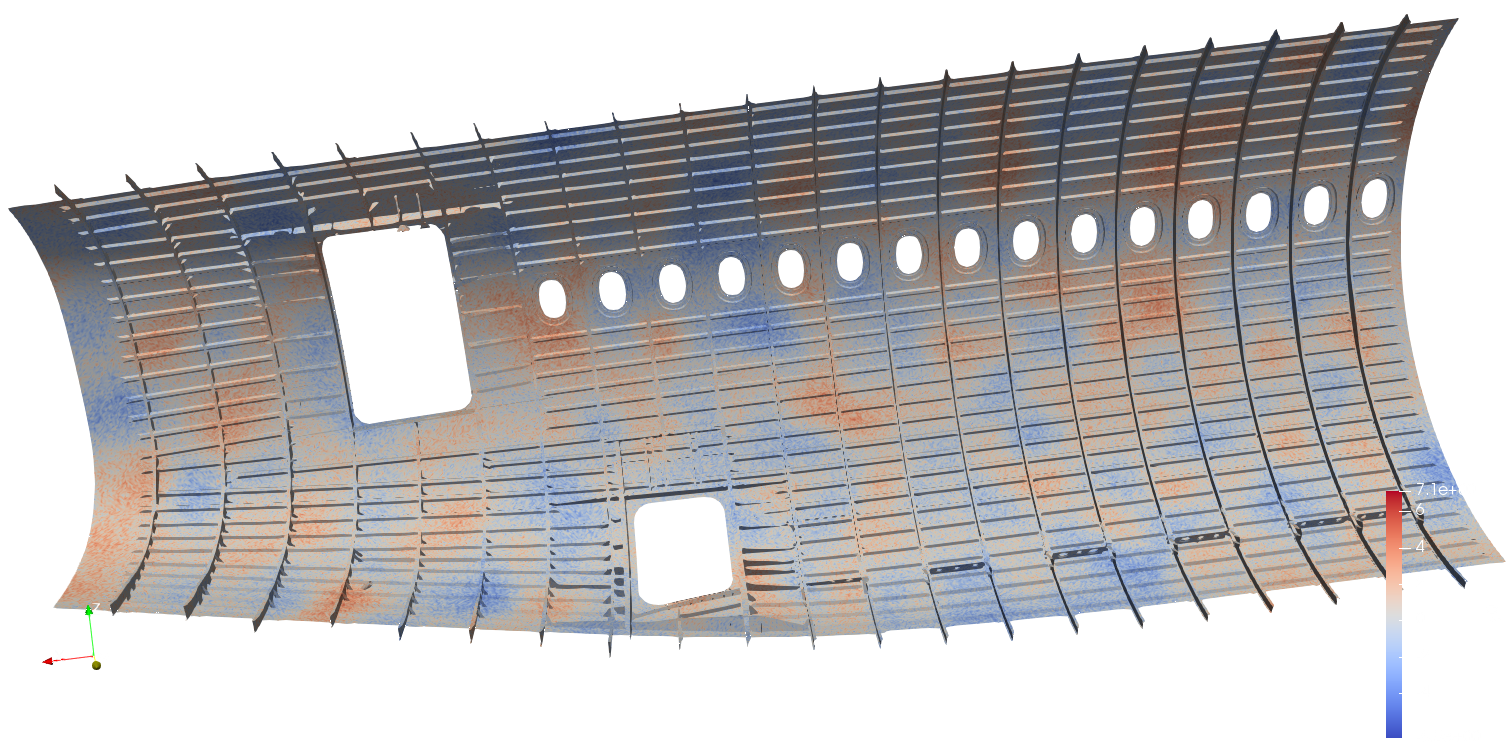
\includegraphics[width=0.8\textwidth]{figures/large_hmat.png}
\end{center}
\caption{SquaredExponential model, 900720 nodes, HMAT (610 s)}
\end{figure}

\begin{figure}
\begin{center}
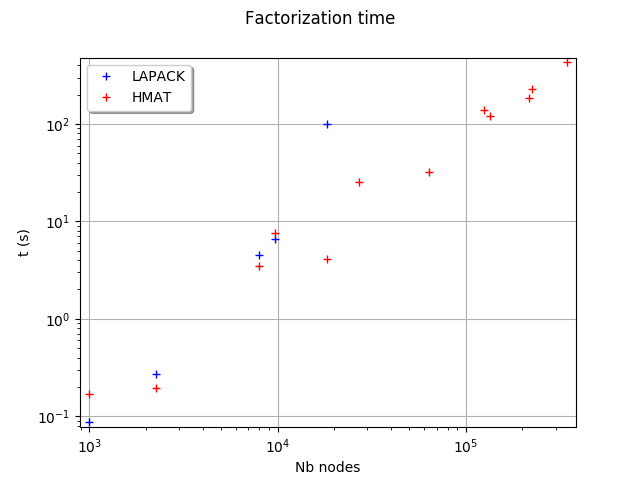
\includegraphics[width=0.45\textwidth]{figures/Factorization.png}%
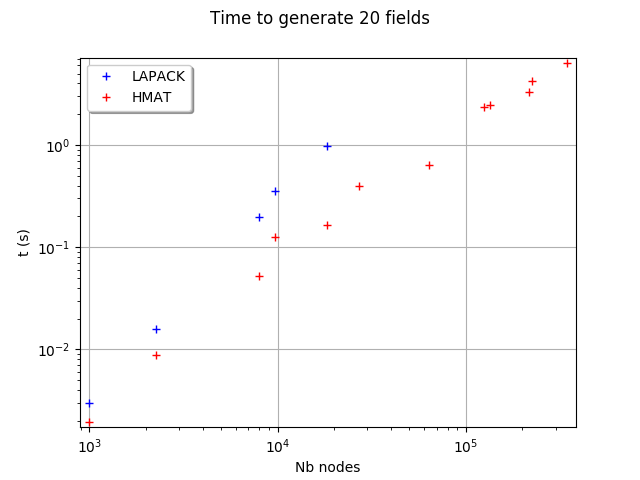
\includegraphics[width=0.45\textwidth]{figures/Sampling.png}
\end{center}
\caption{Factorization time (left) and sampling time (right), lower is better}
\end{figure}

\end{frame}

\begin{frame}[allowframebreaks, containsverbatim]
\frametitle{Karhunen-Loeve decomposition}

The Karhunen-Loeve decomposition of a covariance model on a mesh results in the eigen decomposition of a dense matrix $M=CG$ where $G$ is a sparse matrix, the Gram matrix of the $P_1$ basis over the mesh, and $C$ a dense, positive symmetric definite matrix, the discretization of the covariance model on the mesh.

\begin{itemize}
\item A naive approach is to compute $M$ and to decompose it, which was the only option up to OpenTURNS 1.14.
\item Using an iterative algorithm for the eigen decomposition, the product $z=Mx$ for a given vector $v$ can be done using two products $y=Gx$ and $z=Cy$, both allowing for optimizations.
\end{itemize}

We rely on the \alert{spectra} library (https://github.com/yixuan/spectra) for the iterative algorithm, we use a compressed sparse column compression scheme for $G$ and an hmat compression for $C$ (no regularization/factorization step here).

\alert{Bonus: using spectra, one can select the maximum number of modes to be computed. Here we choose to compute 20 modes}.

\begin{figure}
\begin{center}
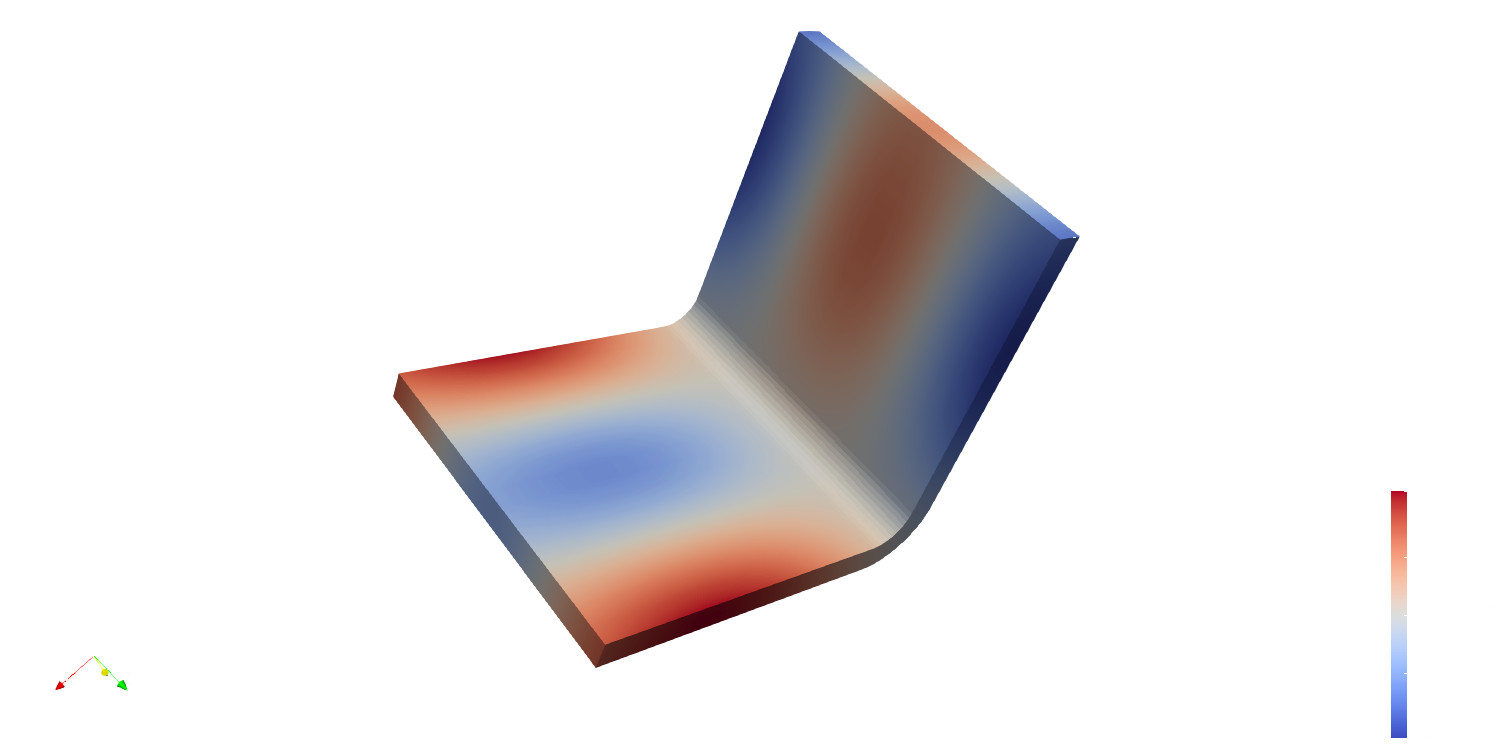
\includegraphics[width=0.5\textwidth]{figures/kl_lapack.png}%
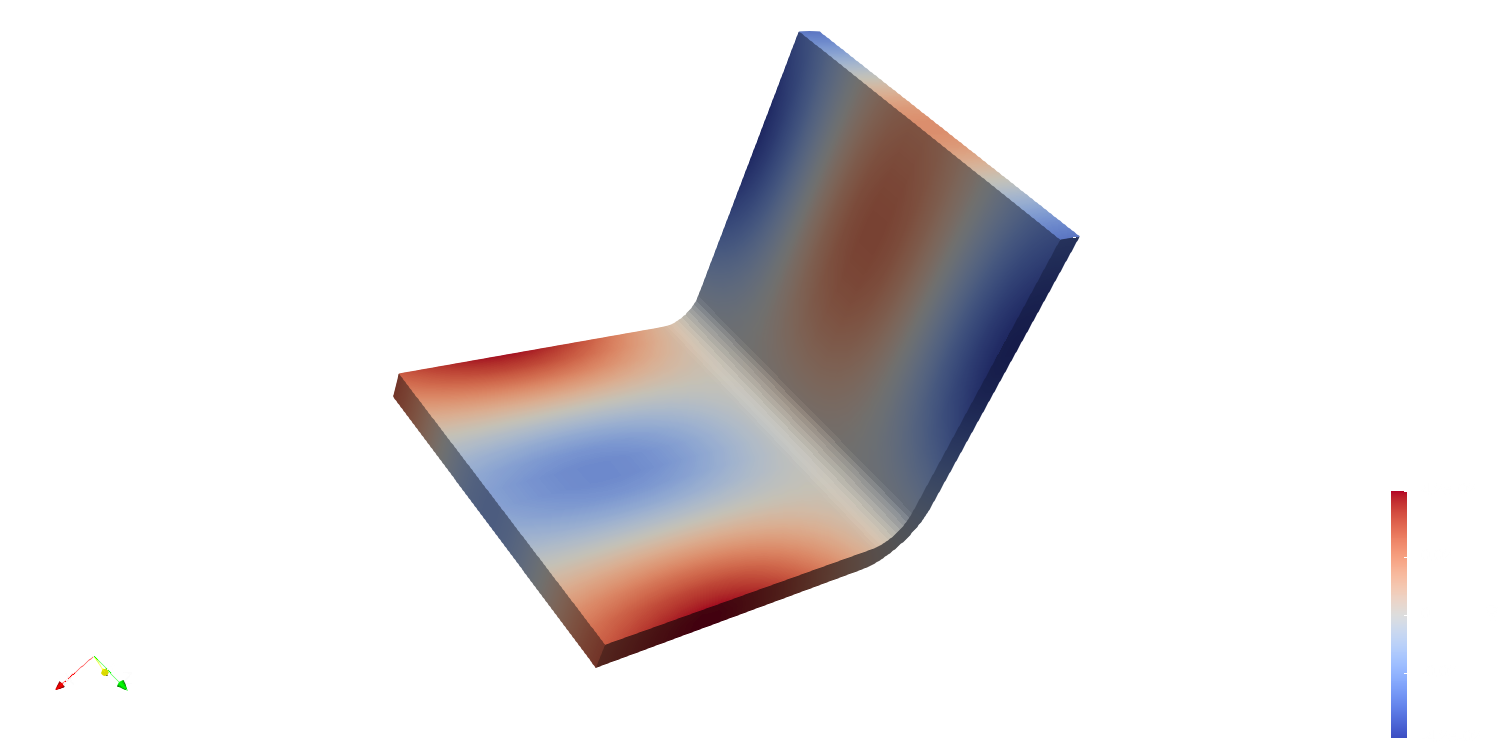
\includegraphics[width=0.5\textwidth]{figures/kl_hmat.png}
\end{center}
\caption{SquaredExponential model, 2268 nodes, mode 11, LAPACK (left, 15.3 s), HMAT (right, 0.1 s)}
\end{figure}

\begin{figure}
\begin{center}
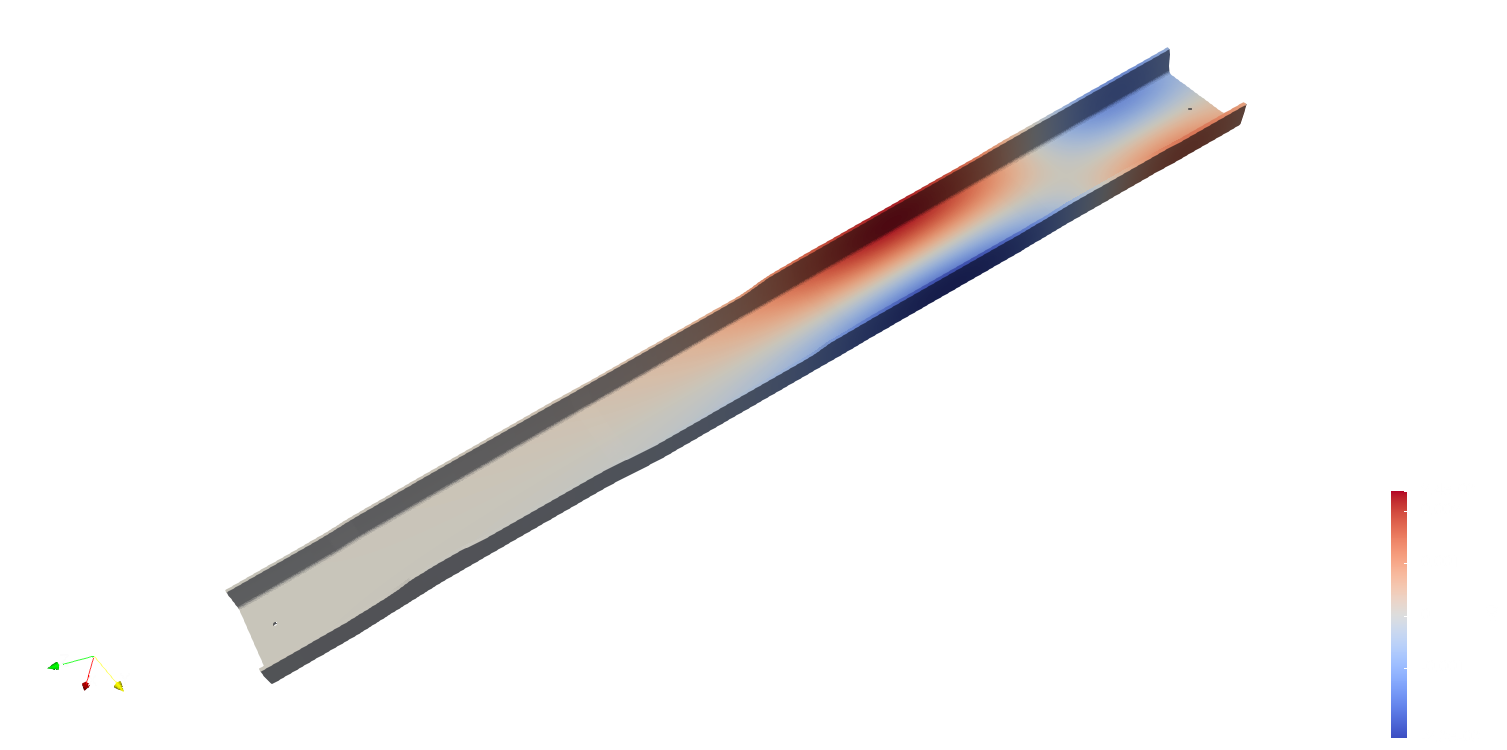
\includegraphics[width=0.8\textwidth]{figures/kl_large_hmat.png}
\end{center}
\caption{SquaredExponential model, 224515 nodes, HMAT (30.1 s)}
\end{figure}

\begin{figure}
\begin{center}
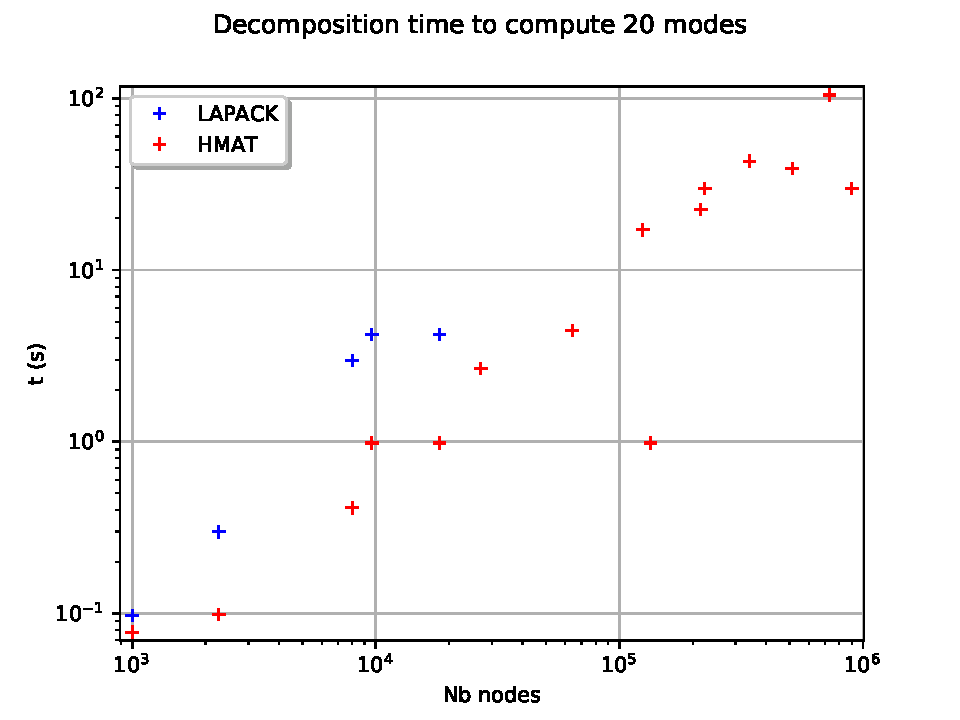
\includegraphics[width=0.8\textwidth]{figures/Decomposition.pdf}
\end{center}
\caption{Decomposition time using spectra and either LAPACK of HMAT}
\end{figure}

\end{frame}


%%%%%%%%%%%%%%%%%%%%%%%%%%%%%%%%%%%%%%%%%%%%%%%%%%%%%%%%%%%%%%%%%%%%%%%%%%%%%
\section{Optimization solvers}

%%%%%%%%%%%%%%%%%%%%%%%%%%%%%%%%%%%%%%%%%%%%%%%%%%%%%%%%%%%%%%%%%%%%%%%%%%%%%

\begin{frame}
\frametitle{Optimization solvers}


\begin{itemize}
\item Dlib (continuous, general-purpose: CG, BFGS, LBFGS, Newton, GLOBAL, LSQ, TrustRegion)
\item Ipopt (continous, large dimension)
\item Bonmin (mixed, large dimension: NLP BB, Outer-approx decomp, Quesada and Grossmann’s BC, Hybrid outer-approx BC, Iterated feasibility pump)
\end{itemize}

%     \column{0.4\textwidth}
% 
\begin{center}
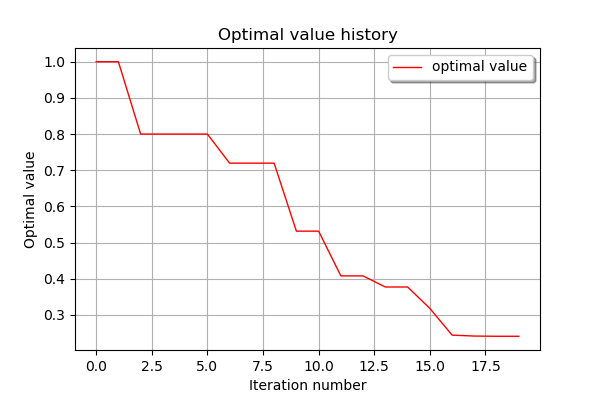
\includegraphics[width=0.7\textwidth]{figures/optim.png}
\end{center}

\end{frame}


% \begin{frame}[containsverbatim]
% \frametitle{Optimization solvers}
% 
% \lstset{language=python}
% 
% \begin{itemize}
% \item Algorithms
% \end{itemize}
% \begin{lstlisting}
% 
% \end{lstlisting}
% 
% \end{frame}

%%%%%%%%%%%%%%%%%%%%%%%%%%%%%%%%%%%%%%%%%%%%%%%%%%%%%%%%%%%%%%%%%%%%%%%%%%%%%
\section{Miscellaneous}

%%%%%%%%%%%%%%%%%%%%%%%%%%%%%%%%%%%%%%%%%%%%%%%%%%%%%%%%%%%%%%%%%%%%%%%%%%%%%

\begin{frame}
\frametitle{Performance improvements}

%   \begin{columns}
%     \column{0.6\textwidth}

\begin{itemize}
% \item HMat new AcaRandom compression method
% \item new Karhunen-Loeve option for efficient SVD with Spectra
\item TBB/OpenBLAS parallel regions conflict: huge penalty
\item TBB-enabled Windows binaries
\item KernelMixture.computePDF ~x10 speed
\item Speed-up Tensor metamodel evaluation: ~x2
\item ODE solvers speedup
\item Memory leaks in Python/SWIG layer
\end{itemize}

%     \column{0.4\textwidth}
% 
% 	\begin{center}
% 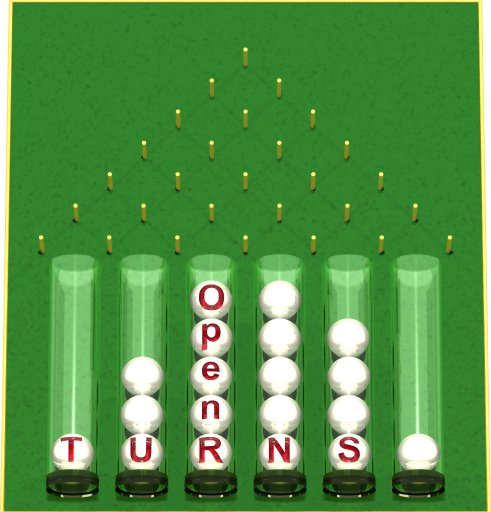
\includegraphics[width=0.9\textwidth]{figures/logo-ot}
% \end{center}

% 	\end{columns}
\end{frame}


\begin{frame}[containsverbatim]
\frametitle{Python layer improvements}

\lstset{language=python}

\begin{itemize}
\item Sample improvements
\end{itemize}
\begin{lstlisting}
x = ot.Sample([[42.0]*3]*8)

# by description marginal accessors
x.getMarginal(['v1', 'v2'])

# get points #2, #5, #6
x[[2, 5, 6]]

# __contains__ operator
[42]*3 in x
=> True
\end{lstlisting}

\end{frame}


\begin{frame}
\frametitle{Other improvements}

%   \begin{columns}
%     \column{0.6\textwidth}

\begin{itemize}
\item Documentation: added examples
\item Bugfixes (and reports), lots of them!
\item Gitter chat
\item New version of otagrum module
\end{itemize}

%     \column{0.4\textwidth}
% 
% 	\begin{center}
% 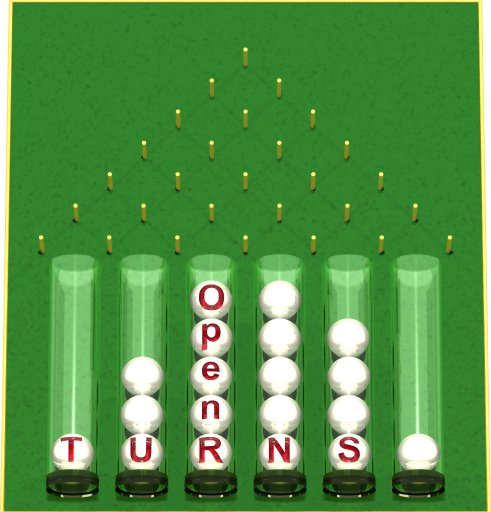
\includegraphics[width=0.9\textwidth]{figures/logo-ot}
% \end{center}

% 	\end{columns}
\end{frame}


%%%%%%%%%%%%%%%%%%%%%%%%%%%%%%%%%%%%%%%%%%%%%%%%%%%%%%%%%%%%%%%%%%%%%%%%%%%%%

% \begin{frame}[containsverbatim]
% 
% Overview :
%   \begin{columns}
%     \column{0.5\textwidth}
% \frametitle{\ot{}}
% \begin{itemize}
% \item First release: 2007
% \item technical committee (including 4 developers), steering committee
% \item Users: mainly in France
% \item Number of users: $\approx 1000$ (10900 Conda downloads in 2016-2017)
% \end{itemize}
% 
%     \column{0.5\textwidth}
% 
% \frametitle{\ot{}}
% \begin{itemize}
% \item Size of the project (2017): 5420 files, 680 classes, 158k sloc
% \item Documentation: theoric, API, developer
% \end{itemize}
% 
% \end{columns}
% 
% \end{frame}

%%%%%%%%%%%%%%%%%%%%%%%%%%%%%%%%%%%%%%%%%%%%%%%%%%%%%%%%%%%%%%%%%%%%%%%%%%%%%

% \begin{frame}[containsverbatim]
% \frametitle{Features overview 1/2}
% 
%   \begin{columns}
%     \column{0.5\textwidth}
% Data analysis:
% \begin{itemize}
% \item Visual analysis
% \item (Non)parametric estimation
% \item Distribution fitting tests
% \item Bayesian calibration
% \end{itemize}
% 
%     \column{0.5\textwidth}
% 
% Probabilistic modeling:
% \begin{itemize}
% \item Dependence modeling: Copulas
% \item Univariate \& multivariate distributions
% \item Process: ARMA, Gaussian
% \end{itemize}
% 
% \end{columns}
% 
% \end{frame}


%%%%%%%%%%%%%%%%%%%%%%%%%%%%%%%%%%%%%%%%%%%%%%%%%%%%%%%%%%%%%%%%%%%%%%%%%%%%%

% \begin{frame}[containsverbatim]
% \frametitle{Features overview 2/2}
% 
%   \begin{columns}
%     \column{0.5\textwidth}
% Meta modeling:
% \begin{itemize}
% \item Gaussian process regression (Kriging)
% \item Spectral methods: Functional chaos expansion, Karhunen-Loeve, low-rank tensors
% \end{itemize}
% 
%     \column{0.5\textwidth}
% 
% Reliability, sensitivity:
% \begin{itemize}
% \item Monte Carlo, LHS, low-discrepancy sequences
% \item Variance reduction methods: importance sampling, subset sampling
% \item Approximation methods: FORM, SORM
% \item Indices: Spearman, Sobol, ANCOVA
% \end{itemize}
% 
% \end{columns}
% 
% \end{frame}


%%%%%%%%%%%%%%%%%%%%%%%%%%%%%%%%%%%%%%%%%%%%%%%%%%%%%%%%%%%%%%%%%%%%%%%%%%%%%

% \section{Example}
% 
% \begin{frame}[containsverbatim]
% \frametitle{Flood example 1/5}
% 
% The flood model of a river compares the water level to the dike height:
% 
% $$S = \left(\frac{Q}{Ks\times300\times\sqrt{(Zm-Zv)/5000}}\right)^{3/5}+Zv-55.5-3$$
% 
% 
% \begin{center}
% 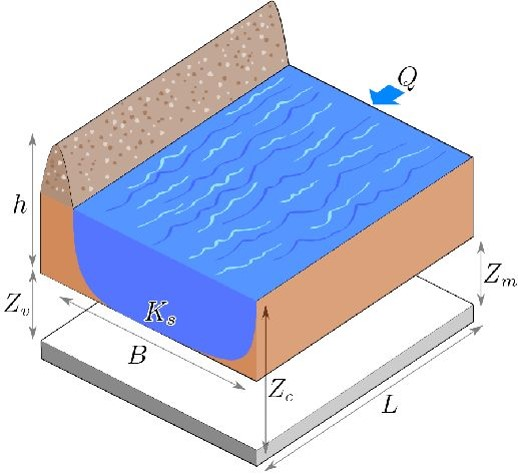
\includegraphics[width=0.5\textwidth]{figures/crue}
% \end{center}
% 
% \end{frame}

%%%%%%%%%%%%%%%%%%%%%%%%%%%%%%%%%%%%%%%%%%%

% \begin{frame}[containsverbatim]
% \frametitle{Flood example 2/5}
% 
% \begin{itemize}
% \item Q $\sim$ Gumbel(alpha=0.00179, beta=1013), flow rate [$m^3s^{-1}$]
% \item Ks $\sim$ Normal(mu=30.0, sigma=7.5), strickler [$m^{1/3}s^{-1}$]
% \item Zv $\sim$ Uniform(a=49, b=51), downstream depth [m]
% \item Zm $\sim$ Uniform(a=54, b=56), upstream depth [m]
% \end{itemize}
% 
% Failure occurs when S is positive, lets estimate $P_f ={\mathbb P}\left( S(\underline{X}) > 0 \right)$.
% 
% \end{frame}
% 
% \begin{frame}[containsverbatim]
% \frametitle{Flood example 3/5}
% 
% \lstset{language=python}
% 
% \begin{lstlisting}
% # Probabilistic model
% Q = ot.Gumbel(1./558., 1013.)
% Ks = ot.Normal(30.0, 7.5)
% Zv = ot.Uniform(49.0, 51.0)
% Zm = ot.Uniform(54.0, 56.0)
% copula = ot.IndependentCopula(4)
% dist = ot.ComposedDistribution([Q, Ks, Zv, Zm], copula)
% \end{lstlisting}
% 
% \begin{center}
% 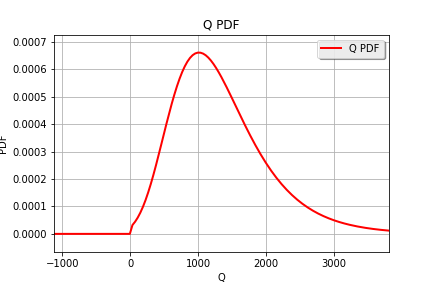
\includegraphics[width=0.5\textwidth]{figures/q_dist}
% \end{center}
% 
% \end{frame}





% 
% \begin{frame}[containsverbatim]
% \frametitle{Flood example 4/5}
% 
% \lstset{language=python}
% \begin{lstlisting}
% # Random variable S=G(Q,Ks,Zv,Zm)
% rv = ot.RandomVector(dist)
% f = ot.SymbolicFunction(['Q', 'Ks', 'Zv', 'Zm'],
%   ['(Q/(Ks*300.*sqrt((Zm-Zv)/5000)))^(3.0/5.0)+Zv-55.5-3.'])
% S = ot.CompositeRandomVector(f, rv)
% \end{lstlisting}
% 
% \begin{center}
% 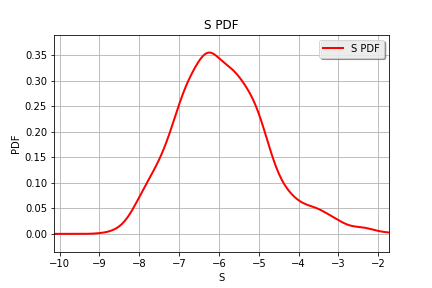
\includegraphics[width=0.5\textwidth]{figures/s_dist}
% \end{center}
% 
% \end{frame}
% 
% 
% 
% 
% 
% 
% 
% 
% \begin{frame}[containsverbatim]
% \frametitle{Flood example 5/5}
% 
% \lstset{language=python}
% \begin{lstlisting}
% # Compute P(S>0) using First Order Reliability Method algorithm
% event = ot.Event(S, ot.Greater(), 0.0) # event S>0
% optimAlgo = ot.Cobyla()
% algo = ot.FORM(optimAlgo, event, dist.getMean())
% algo.run()
% result = algo.getResult()
% print('Pf=', result.getEventProbability()) # P(S>0)=0.00053
% result.drawImportanceFactors()
% \end{lstlisting}
% 
% \begin{center}
% 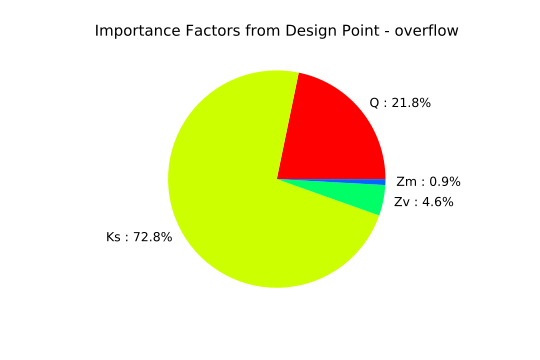
\includegraphics[width=0.6\textwidth]{figures/imp_fact}
% \end{center}
% 
% \end{frame}
% 
% %%%%%%%%%%%%%%%%%%%%%%%%%%%%%%%%%%%%%%%%%%%%%%%%%%%%%%%%%%%%%%%%%%%%%%%%%%%%%
% 
% \section{Software architecture}
% 
% \begin{frame}[containsverbatim]
% \frametitle{Architecture}
% 
% \begin{itemize}
% \item C++ core / SWIG Python bindings
% \item BLAS / LibXml2 / TBB / muParser / NLopt
% \item Packaging: Debian, Conda, Windows
% \item Compilation: cmake
% \item Documentation: Sphinx
% \item Repository: https://github.com/openturns
% \end{itemize}
% 
% \end{frame}
% 
% 
% %%%%%%%%%%%%%%%%%%%%%%%%%%%%%%%%%%%%%%%%%%%%%%%%%%%%%%%%%%%%%%%%%%%%%%%%%%%%%
% 
% \section{Modules}
% 
% \begin{frame}[containsverbatim]
% \frametitle{Modules}
% 
% \begin{itemize}
% \item otrobopt: Robust optimization module
% 
% \item otfmi: FMI models manipulation
% 
% \item otsvm: SVM classifiers, metamodels
% 
% \item otagrum: Bayesian networks module
% 
% \item otwrapy: wrap external simulation codes
% 
% \item ...
% \end{itemize}
% 
% Contributions welcome!
% 
% \end{frame}

%%%%%%%%%%%%%%%%%%%%%%%%%%%%%%%%%%%%%%%%%%%%%%%%%%%%%%%%%%%%%%%%%%%%%%%%%%%%%

\begin{frame}
\frametitle{END}

Thank you for your attention!

Any questions?

\begin{center}
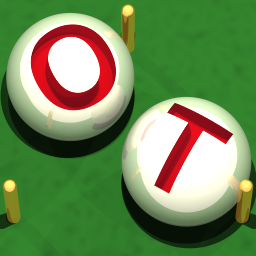
\includegraphics[width=0.2\textwidth]{figures/logo-ot-small}
\end{center}

\end{frame}

% %%%%%%%%%%%%%%%%%%%%%%%%%%%%%%%%%%%%%%%%%%%%%%%%%%%%%%%%%%%%%%%%%%%%%%%%%%%%%
% 
% \section{Bibliography}
% 
% \begin{frame}
% \frametitle{Bibliography}
% 
% \begin{itemize}
% \item Airbus, EDF, ONERA, Phimeca Engineering, IMACS.
% OpenTURNS, a scientific library usable as a Python module dedicated to the treatment of uncertainties, 
% \url{www.openturns.org}.
% \item Airbus, EDF, Phimeca Engineering, IMACS. Documentation of OpenTURNS, version 1.9. 
% \url{http://openturns.github.io/openturns/1.9/contents.html}
% \item  Michaël Baudin, Anne Dutfoy, Bertrand Iooss, and Anne-Laure Popelin. 
% OpenTURNS: An Industrial Software for Uncertainty Quantification in Simulation, 
% Handbook of Uncertainty Quantification, 
% pages 1-38. Springer International Publishing, 2016
% \end{itemize}
% 
% \end{frame}

\end{document}
